\documentclass{article}
\usepackage[utf8]{inputenc}
\usepackage{graphicx}

\title{flores}

\begin{document}

\section{Caça às flores}

Damiko precisa fazer uma pesquisa sobre T diferentes tipos de flores para a escola. Para isso ele irá usar o jardim existente em sua casa para colher esses T tipo de flores. Como ele deixou para realizar a pesquisa de última hora, precisa colher as flores de forma rápida e portanto ele necessita de sua ajuda para encontrar a menor área quadrada do jardim que contém todos os tipos de flores (1 a T inclusive).
\\
Sua tarefa é simples, Damiko irá fornecer um mapa do seu jardim no formato de uma matriz NxM onde, em cada posição, há um valor inteiro representando os tipos de flores no local. A interpretação desses valores funciona da seguinte forma: O resto da divisão desse número por 2 é um valor binário onde 1 (true) significa que existe a flor do tipo 1 e 0 (false) significa que não existe a flor tipo 1. Para a verificação da flor to tipo 2 basta fazer o mesmo procedimento, mas agora para o resultado da divisão da operação anterior. Esse ciclo segue até que o resultado da divisão seja 0.
\\
Portanto se uma posição do jardim contém, por exemplo, o valor 5, isso significa que existem dois tipos de flores: o tipo 1 e o tipo 3. Caso o valor seja 7 ela contém os tipos:  1, 2 e 3. Caso seja 0, não existem flores no local.
Segue um exemplo de mapa 3x4 de um jardim com T=5 tipos de flores:
\\
\begin{center}
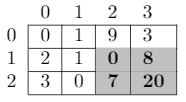
\includegraphics[width=120]{floresTabela.PNG}
\end{center}
\\ \\
No exemplo do jardim acima a menor região que contém os 5 tipos diferentes de flores é a de área 4 destacada iniciando na posição (1, 2) e finalizando na posição (2, 3).

\section*{Entrada}

Na primeira linha serão fornecidos as dimensões $N$ e $M$ do jardim e a quantidade $T$ de tipos de flores a serem pesquisadas por Damiko. Nas $N$ linhas seguintes serão fornecidos $M$ valores $X_{ij}$ que representam os tipos de flores em cada posição do jardim.

\section*{Saída}

Mostre qual a menor área quadrada que Damiko deverá analisar para encontrar todos os tipos de flores de 1 a $T$ e sua coordenada superior esquerda. Caso exista mais de uma resposta possível, exiba a com menor linha. Caso ainda exista mais de uma possível resposta, exiba a com menor coluna. Caso não seja possível encontrar todos os tipos de flores, exiba apenas o valor -1.

\section*{Restrições}

$$1 \leq N,M \leq 500$$
$$1 \leq T \leq 10$$
$$0 \leq X_ij \leq 1023$$

\section*{Exemplos}
\exemplo
